\subsection{نظام الاتصال}
\subsubsection{طوبولوجيا الشبكة}
على مستوى طبقة الـ Data Link، فلدينا العديد من الخيارات المُتاحة. قمنا في البداية بالعمل على بروتوكول ESP-NOW المُطوّر من قبل Espressif، وإنّ الاتّصال اعتماداً على هذا البروتوكول هو اتّصال موثوق TCP من دون الحاجة إلى عمليّات المُصافحة.
نظراً لأهميّة موثوقيّة الاتّصال فقد قمنا باختبار البروتوكول ESP-NOW (one to many) على خمس عقد، حيث تكون أحد العقد هي الـ Master والبقيّة Slaves كما هو موضّح في الشّكل \ref{fig:fig161}.
\begin{figure}
	\centering
	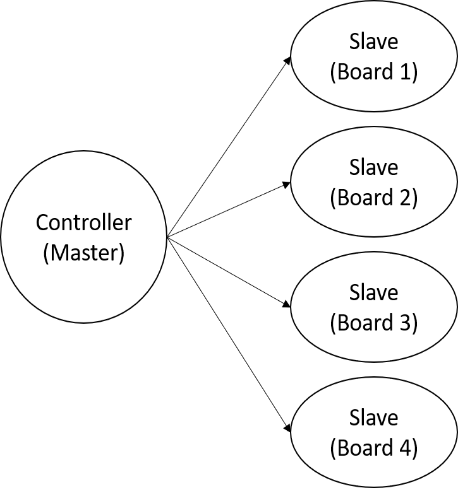
\includegraphics[width=0.4\linewidth]{figs/16/fig16_1}
	\caption{}
	\label{fig:fig161}
\end{figure}


يث قمنا في البداية بتعريف عنوان الـ MAC الخاص بكلّ شريحة اتّصال، ومن ثمّ إرسال إحداثيين x و y مولّدين عشوائياً لجميع العقد ألف مرّة وإعادة التّجربة من أجل أزمنة تأخير مُختلفة كما هو موضّح في الشّكل \ref{fig:fig162}، حيث يمثّل المحور الأفقي أزمن التأخير من أجل الشّرائح  الأربعة، أمّا المحور الشّاقولي فهو عبارة عن الرّسائل الألف المرسلة مُرتّبة من الرسالة الأولى في الأسفل إلى الرسالة الأخيرة في الأعلى.  يُعبّر اللّون الأحمر عن وصول الرّسالة فيما يشير الأسود إلى فشل تسليم الرّسالة.

\begin{figure}
	\centering
	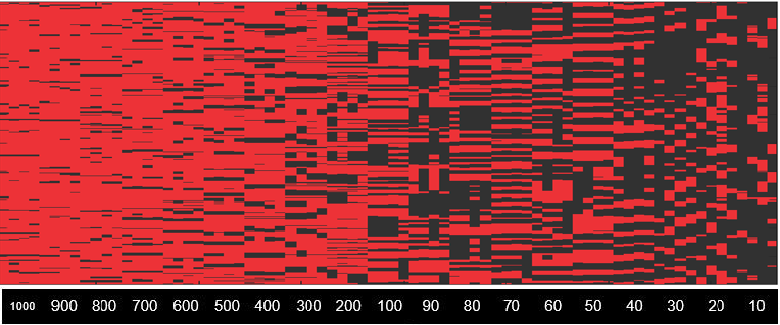
\includegraphics[width=0.9\linewidth]{figs/16/fig16_2}
	\caption{}
	\label{fig:fig162}
\end{figure}

\subsection{بروتوكول $ MQTT $}

هو بروتوكول نقل رسائل بين مخدّم زبون Client/Server بنمط نشر/اشتراك publish/subscribe قائم على الموضوع (Topic)؛ لأنّها ذات تطبيق مستقرّ للـ ESP8266  (باستخدام مخدّم Mosquitto MQTT) حسب [18]. وهنا يجب التّنويه لوجود ثلاث أنماط أساسيّة الاشتراك: النمط القائم على الموضوع والنمط القائم على المحتوى والنمط القائم على النوع.

إنّ بروتوكول MQTT (الموضح في الشكل \ref{fig:fig163}) يتكوّن من ثلاث أجزاء أساسيّة: المخدّم، النّاشر، والمشترك. يُعدّ المخدّم مسؤولاً عن إدارة شبكة من العملاء والّذين هم عبارة عن مزيج من النّاشرين والمشتركين؛ حيث أن النّاشر هو الجهاز الّذي يقوم بإرسال الرّسائل إلى المخدّم بحيث تكون هذه الرّسائل معنونة بعنوان موضوع (topic) بينما المشترك هو الجهاز الّذي يستمع لموضوع أو مواضيع معيّنة. يُمكن تشبيه الموضوع بوسم خاصّ بكلّ رسالة، ويمكن أن يكون وحيد الطّبقة أو متعدّد الطّبقات ويسمح هذا بتقسيم منطقي جيّد للمعطيات. على كلّ جهاز يرغب باستقبال موضوع معين أن يشترك به وذلك بإخبار المخدّم.
\begin{figure}
	\centering
	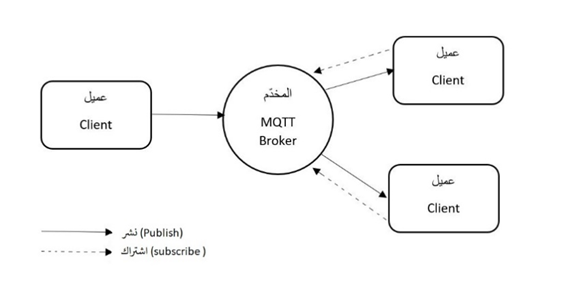
\includegraphics[width=0.7\linewidth]{figs/16/fig16_3}
	\caption{شكل توضيحي للأجزاء الأساسيّة في بروتوكول نقل الرّسائل MQTT}
	\label{fig:fig163}
\end{figure}

ليس هناك اتّصال مباشر بين المشترك والنّاشر وإنّما وببساطة يقوم المشترك بإخبار المخدّم أنّه مهتمّ بمواضيع محدّدة وبعد ذلك يقوم المخدّم بإرسال الرّسائل إلى المشتركين عند توافرها. إنّ نمط نشر/اشتراك مختلف تماماً عن نمط طلب/ردّ (request/response) المتّبع في بروتوكول الـ HTTP. كما أنّ بروتوكول الـ MQTT يعمل بالاعتماد على TCP/IP وعلى خلاف الـ HTTP فهو بروتوكول Binary وليس ASCII، وهذه إحدى ميّزاته فكما نعلم أنّ بروتوكولات الـ binary تستهلك كميّة نقل بيانات أقلّ من الشّبكة. بالإضافة إلى ذلك فهناك خيارات في بروتكول الـ MQTT تتعلّق بتوصيل الرّسالة بين المخدّم والعميل يُطلق عليها QoS (Quality of Service)، وهناك ثلاث خيارات بخصوص هذا الشّأن:

\begin{itemize}
	\item مستوى 0 (QoS = 0): توصيل الرّسالة مرّة واحدة في أفضل حالة؛ أيّ أنّه في حال لم يستلم المشترك الرّسالة فإنّ المُخدّم لن يقوم بإرسالها مرّة أخرى حيث لا يتوقّع المخدّم من المشترك تأكيد وصول الرّسالة (Acknowledgment).
	
	\item مستوى 1 (QoS = 1): توصيل الرّسالة مرّة واحد على الأقلّ. هذا يعني أنّ المخدّم يستمرّ بإرسال الرّسالة إلى أن يقوم المشترك باستلام الرّسالة ويرسل تأكيد باستلامها، وهذا يؤدّي إلى إمكانية وصول أكثر من رسالة واحدة إلى نفس المشترك.
	
	\item مستوى 2 (QoS=2): توصيل الرّسالة مرّة واحدة لزوماً، وهذا يعني أنّ الرّسالة يجب أن تصل لمرّة واحدة ودون تكرار المشترك.
	
\end{itemize}

وفي حال عدم اتّصال المشترك أساساً فيمكننا ضبط الإعدادات بحيث يبدأ الاتّصال بجلسة اتّصال نظيفة؛ حيث يقوم المُخدّم بتجاهل الرّسائل القديمة ويبدأ جلسة جديدة. بينما في حال تعطيل هذه الخاصيّة فإنّ الرسائل (من المستويين 0 و1) الّتي تمّ إرسالها إلى أحد المشتركين أثناء انقطاعه عن الشّبكة سوف تتراكم وسيقوم المُخدّم بإرسالها له فور اتّصاله بالشّبكة.